\chapter{Introduction}
\label{sec:intro}
\pagenumbering{arabic} % para empezar la numeración de página con números

\section{General context}

% An Unmanned Aerial Vehicle (UAV) is an aircraft able to fly without any pilot or operator on board. They may be operated through remote control by a human operator or with various degrees of autonomy, from sensor-driven control aids provided to the operator to fully autonomous flight through preplanned missions.
% UAVs have existed since the 20th century and were initially developed as military technology to protect pilots from dangerous missions.
% However, as the cost of the electronics and sensors decreased and control technologies improved, they became available to a broader public. They are now employed in various civil applications like crop control, search and rescue, or filmmaking and photography.
% Most commercial solutions are limited to remote operations or rudimentary autonomy, with fully autonomous flight still in the earliest phases.
% However, there is a growing trend towards using vision-based control solutions, which can offer improved performance and flexibility compared to traditional control methods.

% Vision-based control solutions use cameras and image processing algorithms to provide real-time feedback and control of the UAV. 
% These solutions are often more flexible and robust than traditional control methods, which are typically based on accelerometers, gyroscopes, and other sensors. 
% Additionally, vision-based control solutions can be implemented on low-cost platforms, making them accessible to a broader range of users.
% These vision-based guidance systems have only started to appear in recent years as artificial intelligence becomes more widespread and very few fully-developed consumer-ready platforms are available for the general public.
% Even so,
% from the essential hardware to build an own quadcopter, a helicopter with four rotors that represents the most common type of UAV, to miniaturized computers that handle complex calculations and open-source software that can be customized to endless applications,
% all the individual pieces that enable building such a system are readily available.

Unmanned Aerial Vehicles (UAVs), commonly known as drones, have emerged as remarkable aircraft capable of flying without a pilot or operator on board. Originally developed as military technology to safeguard pilots from dangerous missions, UAVs have transitioned into the civilian domain due to advancements in control technologies and the decreasing costs of electronics and sensors. This has led to broader accessibility of UAVs, allowing their utilization in diverse civil applications such as crop monitoring, search and rescue operations, and filmmaking and photography.
Traditionally, UAVs have been operated either remotely by a human operator or with limited autonomy through preplanned missions. However, recent trends have indicated a shift towards vision-based control solutions, which offer promising advantages over conventional control methods. Vision-based control harnesses the power of cameras and image processing algorithms to provide real-time feedback and precise control of UAVs.

Compared to traditional control systems that heavily rely on sensors such as accelerometers and gyroscopes, vision-based control solutions offer greater flexibility and robustness. By leveraging the visual input from cameras, these solutions can adapt to varying environmental conditions and handle complex flight scenarios more effectively. Furthermore, vision-based control methods are often more accessible, as they can be implemented on lower-cost platforms, making them appealing to a wider range of users.
While the integration of vision-based control solutions into UAVs is a relatively recent development, propelled by the increasing prevalence of artificial intelligence, there is limited availability of fully-developed consumer-ready platforms in the market. However, this does not impede progress in this field, as all the necessary components for constructing such systems are readily available. From the essential hardware required to build a quadcopter, which represents the most common type of UAV, to miniaturized computers capable of handling complex calculations, and open-source software that can be customized for endless applications, the individual pieces required for constructing and implementing vision-based control solutions are very accessible.

In summary, the rise of UAVs and their integration into various civil applications has paved the way for the exploration of vision-based control solutions. These solutions, utilizing cameras and image processing algorithms, offer enhanced performance, adaptability, and accessibility compared to traditional control methods. Although consumer-ready platforms are still emerging, the necessary components for constructing vision-based control systems are readily available, fueling the advancement of this field.

\section{The DroneVisionControl project}

% The project presented in this thesis aims to show the tools available to design and implement control solutions for the popular PX4 open-source autopilot platform and how to integrate them with detection and tracking computer vision mechanisms to achieve simple vision-based self-guided UAVs.
% To do that, a simple application has been developed to use as a basis for delving into the PX4 ecosystem and exploring ways of integrating the hardware and software necessary to control a UAV.
% Two main architectures of software and hardware interaction in vision-based scenarios are proposed based on whether the vision module is located offboard or onboard the vehicle during flight.
% The first case, the simpler of the two, will be used as a landing platform to begin development and test the most basic integration between the tools employed, by designing a proof-of-concept control mechanism that translates hand gestures executed in front of an independent camera to flight commands that control the movement of the vehicle.
% The second scenario builds upon the previous one to integrate the camera and vision computation onboard the vehicle to develop a tracking and following control solution that looks for a person standing in the field of view of the drone and mirrors its movements in a 3D environment to keep it on sight.

% This thesis explores the development environment used, which enables a process for designing the software in a way that gradually adapts to the hardware employed by building up progressively from a completely simulated flight controller to actual flight tests in an unmanned vehicle.
% To do that, the AirSim simulation engine is leveraged to build an environment that allows for safe and thorough testing of unreliable, in-progress control solutions.
% All the necessary code for this project has been written in Python and always runs outside the flight controller board on a companion computer.
% This allows more processing power to be accessible for any compute-intensive computer vision algorithms,
% but also ensures that the control solutions are abstracted from the hardware components and not dependent on the specific flight stack employed, 
% to allow applying the results to any available autopilot platform with exposed APIs.

The project outlined in this thesis is a comprehensive exploration of the tools available for designing and implementing control solutions for the PX4 open-source autopilot platform. The goal is to demonstrate how these tools can be integrated with computer vision mechanisms to achieve vision-based self-guided unmanned aerial vehicles (UAVs).
To achieve this objective, a simple application has been developed named Drone Vision Control serving as a foundation for the investigation into the PX4 ecosystem and methods of integrating the necessary hardware and software for UAV control.
For the computer vision detection mechanisms, the ready-to-use Mediapipe suite of libraries for real-time image analyses on hand-held devices has been employed to reduce the complexity of the project.
Two primary architectures for integrating software and hardware in vision-based scenarios have been proposed, with one scenario involving off-board vision modules and the other integrating onboard camera and vision computation. 

The first scenario involves a proof-of-concept control mechanism that translates hand gestures executed in front of an independent camera to flight commands, thereby controlling the movement of the vehicle. This serves as a landing platform to begin development and test the most basic integration between the tools employed.
The second scenario builds on the first to integrate the camera and vision computation onboard the vehicle to develop a tracking and following control solution that can track and follow a person standing in the drone's field of view by mirroring their movements in a 3D environment.

To further the development of these control mechanisms, a dedicated development environment was employed. This environment facilitated the design process by allowing a gradual adaptation of the software to match the hardware requirements, starting from a purely simulated flight controller and progressing towards real flight tests in an unmanned vehicle.
The key component of this environment is the integration with the AirSim simulation engine. Built upon the powerful 3D computer graphics game engine Unreal, it provides a platform that ensures secure and comprehensive testing of control solutions that are still in progress and not yet fully reliable.

For this project, all the code has been implemented in Python, running on a companion computer separate from the flight controller board. This deliberate approach ensures that the control solutions remain independent of the hardware components and are not tied to any particular flight stack. Consequently, the results obtained can be applied to any autopilot platform that offers exposed APIs and are not limited to the PX4 ecosystem. 

In conclusion, this thesis offers a thorough investigation into the development of vision-based self-guided UAVs, presenting a range of tools and techniques that can be utilized to accomplish this objective.

\section{Objectives}
\label{sec:objetives}

The main objective of this project is to explore the tools and methods available for designing and implementing control solutions for the PX4 open-source autopilot platform and demonstrate how they can be integrated with computer vision mechanisms to achieve a self-guided UAV that tracks and follows a person's movements.

More specifically, it aims to:
\begin{itemize}
    % \item Introduce the software and hardware environment of the Dronecode project and the techniques they have made available.
    % \item Show the minimum requirements needed to develop control software for the platform.
    % \item Suggest viable vision-driven control solutions that use those techniques.
    % \item Present a testing process using available tools that can help ensure safety and reliability for any new solutions developed.
    % \item Build a quadcopter and use it to carry out test flights with the developed solutions.
    \item Research and understand the PX4 platform and its wider ecosystem, including its architecture, capabilities, and available APIs.
    \item Explore existing computer vision mechanisms and algorithms suitable for vision-based control of UAVs.
    \item Design and set up a dedicated development environment using the AirSim simulation engine for secure and comprehensive testing of control solutions.
    \item Employ both software-in-the-loop and hardware-in-the-loop simulation approaches to comprehensively evaluate the control solutions in the simulation engine.
    \item Develop a proof-of-concept control mechanism that translates hand gestures captured by a camera into flight commands for the UAV.
    \item Integrate the hand gesture control mechanism with the PX4 platform and test its functionality in a simulated environment.
    \item Investigate hardware and software requirements for integrating onboard cameras and vision computation in UAVs.
    \item Develop a tracking and following control solution that can mirror the movement of a person.
    \item Test the tracking and following control solution in a simulated environment, integrating the onboard camera and vision computation with the PX4 platform.
    \item Conduct flight tests on a self-built quadcopter to evaluate the developed control mechanisms, analyzing their performance and reliability in different scenarios.
    \item Document the findings, methodologies, and results obtained throughout the project and provide recommendations for future improvements.
\end{itemize}


\section{Time planning}
\label{sec:time-planning}

\begin{figure}
  \centering
  \makebox[\textwidth][c]{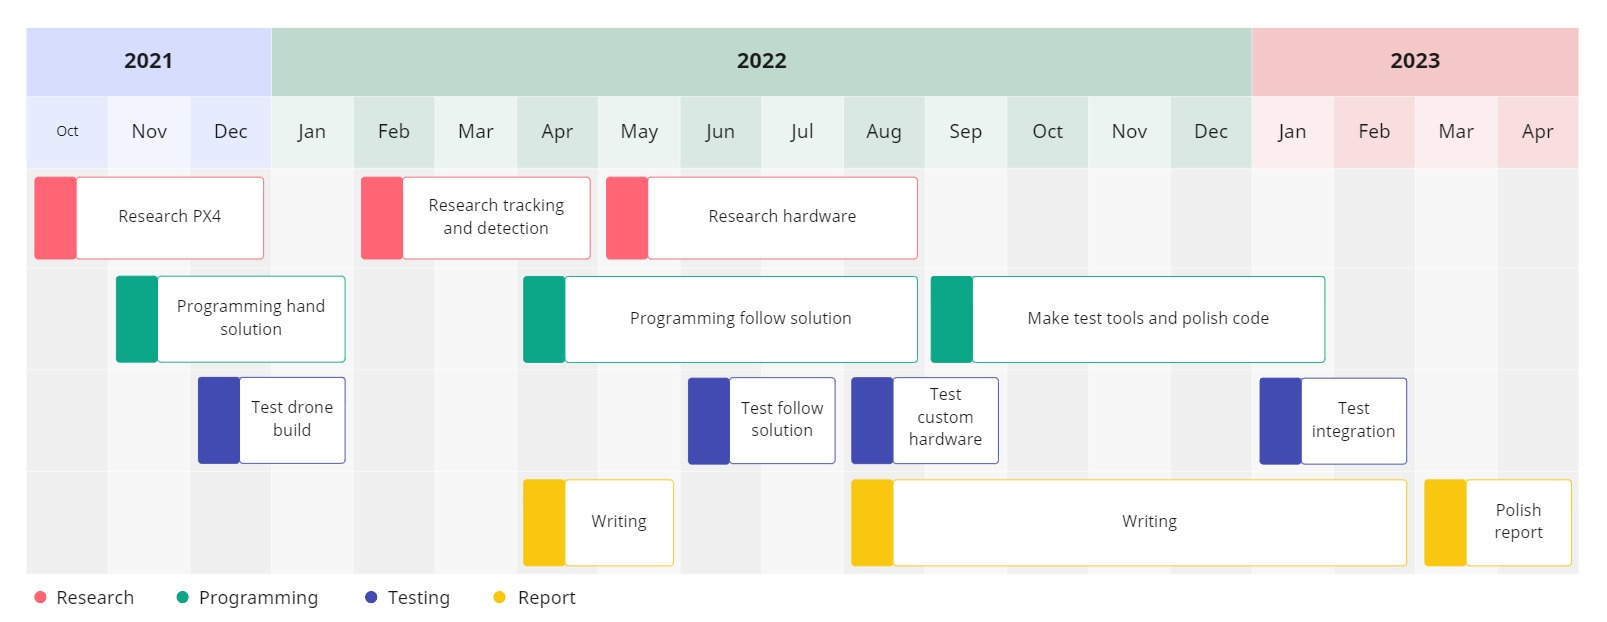
\includegraphics[width=1.1\textwidth,keepaspectratio]{img/project-timeline.jpg}}
  \caption{Timeline for the development of the project}
  \label{fig:project-timeline}
\end{figure}

% This project has been carried out over a natural period of one and a half years due to having to coordinate with working a full-time job in parallel.
% The development has been spread out over three phases, taking up a total of 400 hours of dedication to the project.
% Each of these phases can be divided into three main tasks: research of the necessary systems, programming of custom solutions and tools, and comprehensive testing on different scenarios.
% Additionally, during the last two phases, time was allocated to the process of writing the report, which occurred concurrently with the research and development work.
% \begin{itemize}
%     \item Phase 1: Proof-of-concept ( Oct 21 - Jan 22: 61 hours )
%     \begin{itemize}
%         \item Research PX4 (12 hours)
%         \item Programming hand solution (42 hours)
%         \item Test standard drone build (7 hours)
%     \end{itemize}
%     \item Phase 2: Follow solution ( Feb 22 - Aug 22: 138 hours )
%     \begin{itemize}
%         \item Research tracking and detection (33 hours)
%         \item Programming follow solution (80 hours)
%         \item Test custom hardware (25 hours)
%     \end{itemize}
%     \item Phase 3: Hardware ( Sep 22 - Feb 23: 65 hours )
%     \begin{itemize}
%         \item Research hardware (15 hours)
%         \item Make test tools and polish code (33 hours)
%         \item Test custom hardware and integration (17 hours)
%     \end{itemize}
%     \item Writing report (133 hours)
% \end{itemize}

This project was carried out over a period of approximately one and a half years, taking into account the parallel commitment of working a full-time job. The development process was divided into three distinct phases, totalling approximately 400 hours of dedicated effort. These phases consisted of the following tasks:

\begin{itemize}
\item \textbf{Phase 1: Proof-of-concept (Oct 2021 - Jan 2022: 61 hours)}
\begin{itemize}
\item Conducted research on the PX4 system (12 hours)
\item Programmed the hand solution (42 hours)
\item Tested the standard drone build (7 hours)
\end{itemize}

\item \textbf{Phase 2: Follow solution (Feb 2022 - Aug 2022: 138 hours)}
\begin{itemize}
    \item Conducted research on tracking and detection methods (33 hours)
    \item Developed the follow solution (80 hours)
    \item Tested custom hardware (25 hours)
\end{itemize}

\item \textbf{Phase 3: Hardware (Sep 2022 - Feb 2023: 65 hours)}
\begin{itemize}
    \item Conducted research on hardware options (15 hours)
    \item Developed test tools and refined code (33 hours)
    \item Conducted testing of custom hardware and integration (17 hours)
\end{itemize}
\end{itemize}

During the initial phase, extensive research was conducted to gain a deep understanding of the PX4 system. This involved studying the architecture, capabilities, and documentation of the platform. Following the research phase, a proof-of-concept control mechanism was developed, enabling the translation of hand gestures captured by an independent camera into flight commands. Subsequently, testing was performed on the standard drone build to verify the basic integration between the control mechanism and the UAV platform.

The second phase focused on the development of an advanced tracking and following control solution. Research was conducted to explore various tracking and detection methods, including computer vision algorithms and techniques. Building upon this research, the follow solution was implemented, enabling the UAV to track and follow a person in its field of view by mirroring their movements in a 3D environment. Custom hardware components, such as sensors and actuators, were tested to ensure compatibility and reliable operation within the follow solution.

In the third phase, research was conducted to explore hardware options for the UAV system, including flight controllers, companion computers, and cameras. The chosen hardware components were integrated, and test tools were developed to enhance the performance and reliability of the control mechanisms. The system's hardware and software integration was thoroughly tested to ensure seamless operation and optimize the control algorithms.


Additionally, a significant amount of time, totalling 133 hours, was dedicated to writing the report, which was carried out concurrently with the research and development work.

This time planning and task distribution allowed for a structured approach to the project, ensuring a comprehensive exploration of the subject matter while accommodating other commitments.

\section{Thesis layout}
\label{sec:layout}

% This section details the structure of this thesis.
% It is organized into five chapters that reflect the three distinct tasks described in the last section: research, development and testing, along with this introduction and some final conclusions.
% Specifically:

% \begin{itemize}
%     \item In the first chapter, there is a brief introduction to the context in which the project has been developed, as well as the objectives it pursues.
%     \item Chapter 2 presents the technologies and tools employed in this project and the current state-of-the-art for UAV vision-based control solutions.
%     \item The third chapter introduces the simulation environments used to develop the solutions throughout the project and the architecture of the hardware and software used.
%     \item Chapter 4 follows along through the process of testing every part of the system incrementally until reaching the final flight tests.
%     \item The last chapter shows the conclusions drawn from the work and presents ideas for future development.
% \end{itemize}

The thesis is structured into five chapters, with the three main blocks focusing on each of the three specific aspects of the project mentioned in the previous section: research, development and testing. 

The first chapter serves as an introduction to the context in which the project has been developed, providing background information and highlighting the objectives pursued throughout the research. It sets the stage for the subsequent chapters, giving an overview of the project's scope and purpose.

The second chapter discusses the technologies and tools employed in the project and provides a review of the relevant literature and the current state-of-the-art for UAV vision-based control solutions.

The third chapter covers the simulation environments used throughout the project and the architecture of the hardware and software employed in the project. This chapter discusses the design decisions that went into selecting the hardware and software components and describes the overall architecture of the system.

The fourth chapter presents the testing methodology used throughout the project, from initial simulations to flight tests. This chapter provides a detailed account of the testing process and highlights the key findings and insights gained from each phase of testing.

The final chapter concludes the thesis by summarizing the key findings of the project and drawing conclusions about the effectiveness and limitations of the control system. Additionally, this chapter provides suggestions for future development and improvement of the system.
